
\documentclass[12 pt]{article}


\setlength{\textwidth}{6.3in}
\setlength{\textheight}{9in}
\setlength{\oddsidemargin}{-0.25in}
\setlength{\evensidemargin}{-0.44in}
\setlength{\topmargin}{-0.2in}
\usepackage{graphicx}
\usepackage{epsfig}
\usepackage{epstopdf}

\begin{document}

\title{Media Streaming Workload: Cost-Efficient Elastic Orchestration}
\date{}
\maketitle

Motivation by high amount of video traffic in US (over 50$\%$ streamed from Netflix and YouTube). This incur a lot of cost on streaming service provider which by part can be tenant of a public cloud (e.g. Netflix). Elastic resource provisioning and scaling can save them a lot... We show here x$\%$ reduction in cost by using our proposed mechanism. %Elastreaming

{\bf Popularity vs. Resolution:}\\
Server procurement is highly dependent on the type of content requested by the client and also its popularity. E.g. a popular event like super bowl which is viewed by millions of audiences will be network intensive while needs very little cache (because of high locality among the viewers). On the other hand a high definition content can benefit a lot from more cached frames while network is not an issue for a smooth streaming to the client Figure \ref{fig:spectrum}.
\\

{\bf Clients network condition:} \\
In video streaming applications usually end users can have very different network capacity based on their network provider, congestion level and physical layer (PHY) interference for wifi communications. The video client running on different devices choose their video rate according to estimated network capacity ref[netflix paper].

\begin{figure}[!htb]
\centering
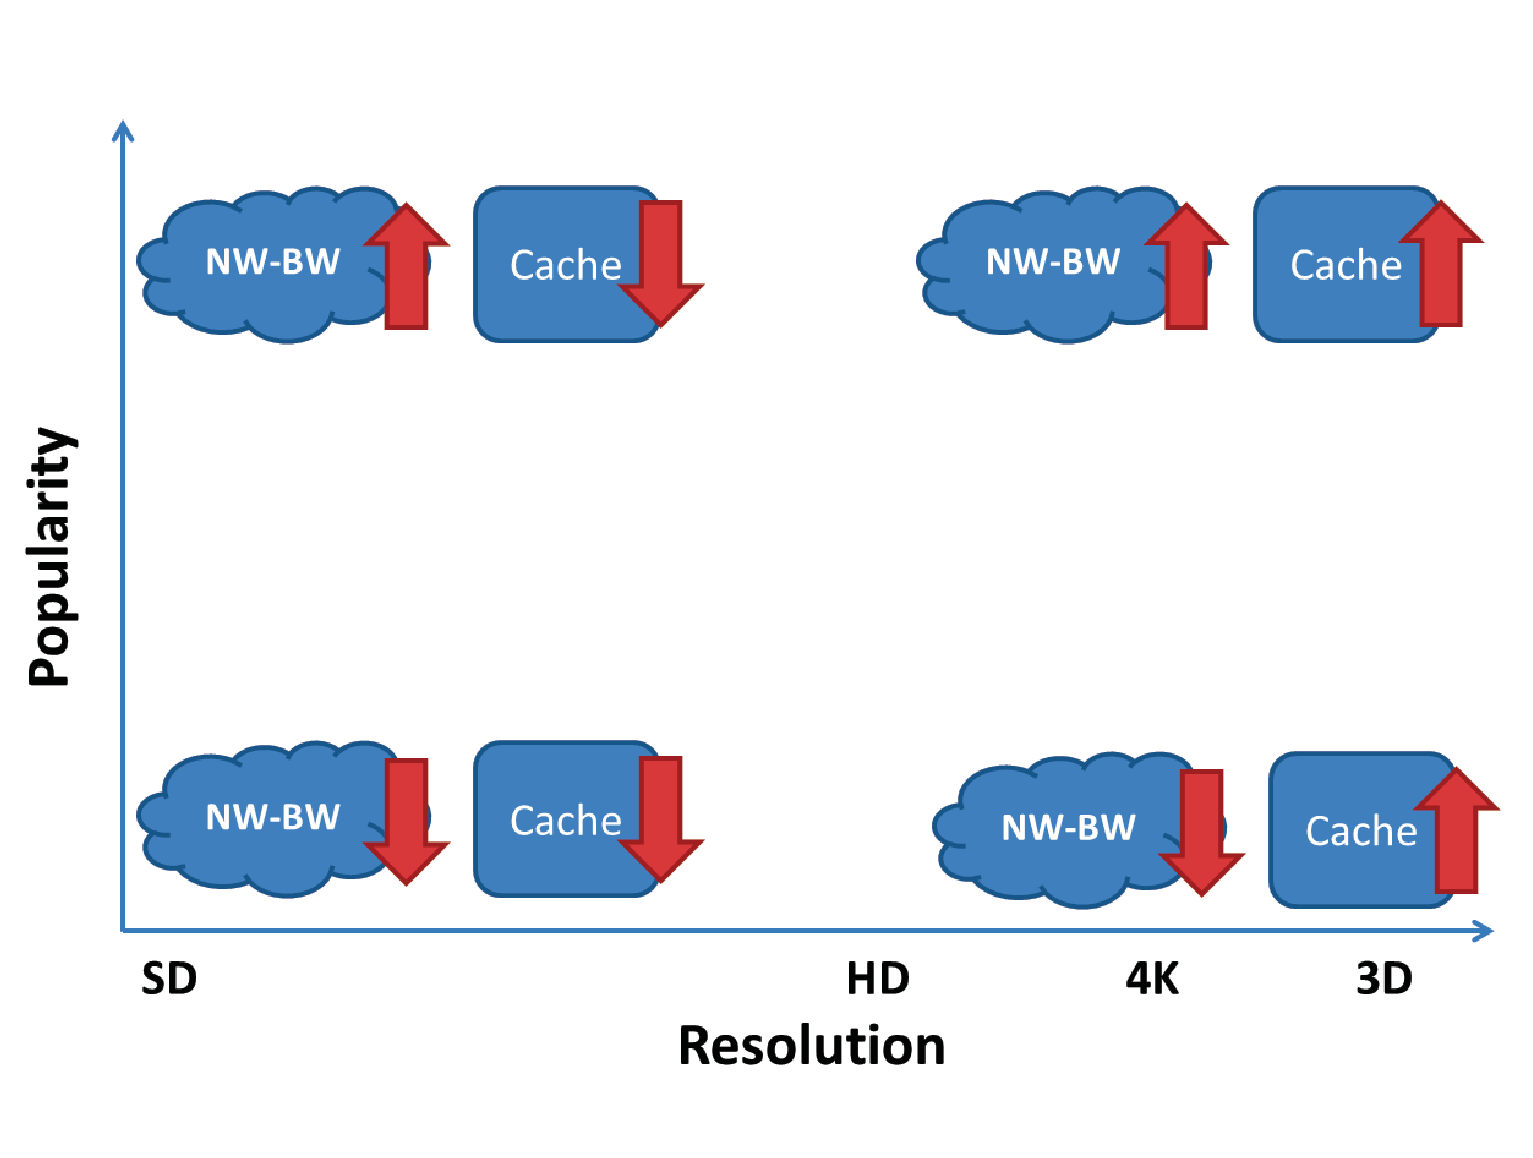
\includegraphics[trim={1cm 0.6cm 5cm 1cm},width=0.4\textwidth]{./spectrum.eps}
\caption{Guideline for resource provisioning for a media streaming server}\label{fig:spectrum}
\end{figure}

{\bf Next Step:} 1) Simple experiment comparing costs vs. performance in following settings: (A) using one VM (B) two VMs with half the RAM capacity, both with low network guarantee. Look at these two cases under realistic pricing (additive) and future pricing (bulk discount model).
Exp expectation: Looking at different clients can result in different results, e.g. if clients are watching a popular content then the (B) should perform better than (A) while it might be more expensive under future pricing. If clients are watching very different content and more RAM is needed then (A) will be a better solution for the server since it is more cost-efficient and result in less interruptions at client side.





\end{document}


